\documentclass[12pt]{article}

\usepackage[a4paper, includefoot,
			left=1cm,
			right=1cm,
			top=2cm,
			bottom=2cm,			
			headsep=1cm,
			footskip=1cm]{geometry}

\renewcommand{\familydefault}{\sfdefault}
\usepackage[T2A]{fontenc}
\usepackage[utf8x]{inputenc}
\usepackage[english]{babel}
\usepackage{babelbib}
\usepackage{hyperref}
\setcounter{tocdepth}{2}
\usepackage{float}
\usepackage{simplewick}

% полуторный интервал во всем документе
\usepackage{setspace}
\onehalfspacing

\usepackage{cite}

% многострочные комментарии
\usepackage{comment}

% for Dirac's bra-ket notation
\usepackage{braket}

% for systems of equations
\usepackage{mathtools}

% for advanced math equations
\usepackage{amsmath}
\usepackage{amsfonts}
\usepackage{bm}

% for left eigenvectors
\newcommand{\Perp}{{\perp\perp}}

% нумерация глубоких подразделов (subsubsection)
\setcounter{secnumdepth}{5}

\usepackage{array}
\newcolumntype{C}[1]{>{\centering}m{#1}}

% для оформления базисных наборов в приложении
\usepackage{listings}
\usepackage{xcolor}
\usepackage{textcomp}
\definecolor{lightlightgray}{gray}{0.93}
\definecolor{darkgreen}{rgb}{0.0, 0.2, 0.13}
\definecolor{codegreen}{rgb}{0,0.6,0}
\lstset{
	backgroundcolor = \color{lightlightgray},
	basicstyle=\small\ttfamily
}

\lstset {
    language=C++,
%    frame=tb,
    tabsize=4,
    showstringspaces=false,
%    numbers=left,
    %upquote=true,
    commentstyle=\color{gray},
    keywordstyle=\color{blue},
    stringstyle=\color{red},
    basicstyle=\small\ttfamily, % basic font setting
    emph={libgrpp_shell_t,libgrpp_potential_t,libgrpp_grpp_t},
    emphstyle={\color{codegreen}},
    %escapechar=\&,
    % keyword highlighting
    classoffset=1, % starting new class
    %otherkeywords={>,<,.,;,-,!,=,~},
    %morekeywords={>,<,.,;,-,!,=,~},
    keywordstyle=\color{blue},
    classoffset=0,
}

\lstset {
    language=Fortran,
%    frame=tb,
    tabsize=4,
    showstringspaces=false,
%    numbers=left,
    %upquote=true,
    commentstyle=\color{gray},
    morecomment=[l][\color{gray}]{!},
    keywordstyle=\color{blue},
    stringstyle=\color{red},
    basicstyle=\small\ttfamily, % basic font setting
    emph={libgrpp_shell_t,libgrpp_potential_t,libgrpp_grpp_t},
    emphstyle={\color{codegreen}},
    %escapechar=\&,
    % keyword highlighting
    classoffset=1, % starting new class
    %otherkeywords={>,<,.,;,-,!,=,~},
    %morekeywords={>,<,.,;,-,!,=,~},
    keywordstyle=\color{blue},
    classoffset=0,
}


% для фиксированной ширины колонок в таблицах
\usepackage{array}
\newcolumntype{L}[1]{>{\raggedright\let\newline\\\arraybackslash\hspace{0pt}}m{#1}}
\newcolumntype{C}[1]{>{\centering\let\newline\\\arraybackslash\hspace{0pt}}m{#1}}
\newcolumntype{R}[1]{>{\raggedleft\let\newline\\\arraybackslash\hspace{0pt}}m{#1}}



%=================================================================================

\begin{document}

% интервал полуторный

\title{
\normalsize

{\large \texttt{libgrpp}}

\bigskip

{\bf a library for the evaluation of molecular integrals \\
of the generalized relativistic pseudopotential operator (GRPP) over Gaussian functions \\
v 1.2.0}

\bigskip

\textit{programmer's manual}

\bigskip

\textit{written by \\
A. Oleynichenko}

\bigskip

\textit{Quantum Physics and Chemistry Department \\
Petersburg Nuclear Physics Institute named by B. P. Konstantinov \\
National Research Centre ``Kurchatov Institute'' \\
Gatchina, Russia}
}
\maketitle

\newpage

\tableofcontents

\newpage

\section{Introduction}

\texttt{libgrpp} is a library of subroutines for the evaluation of molecular integrals of the generalized relativistic pseudopotential operator (GRPP) over Gaussian functions~\cite{Oleynichenko:LIBGRPP:23}.

\subsection{Generalized relativistic pseudopotentials}
Generalized (or Gatchina) relativistic pseudopotentials (GRPPs) of atomic cores imply the use of different semilocal potentials for atomic electronic shells with the same orbital and total momentum quantum numbers but with different principal quantum numbers~\cite{Mosyagin:97,Titov:91,Titov:99}. GRPPs give rise to accurate and reliable relativistic electronic structure models of atoms, molecules, clusters and solids~\cite{Lomachuk:20,Maltsev:21,Shakhova:22}. GRPPs can readily incorporate the effects of Fermi nuclear charge distribution, Breit electron-electron interactions~\cite{Petrov:04,Mosyagin:06} and quantum electrodynamics effects (electron self-energy and vacuum polarization)~\cite{Shabaev:13,Zaitsevskii:QED:22}. GRPPs give rise to very accurate relativistic Hamiltonians at the moment, allowing one to completely bypass any complicated four-component calculations at a price of a very moderate loss of accuracy~\cite{Oleynichenko:LIBGRPP:23}. Generalized pseudopotentials developed in the Quantum Physics and Chemistry Department (NRC ``Kurchatov Institute'' -- PNPI) in the last three decades are available online at \url{http://qchem.pnpi.spb.ru/recp}.

\subsection{Features of \texttt{libgrpp}}

Basis functions:

\begin{itemize}
\item Cartesian contracted GTOs;
\item max angular momentum of basis functions $l_{max} = 10$ (up to $n$-functions, can be increased by hands).
\end{itemize}

\noindent
Pseudopotential integrals:

\begin{itemize}
\item scalar-relativistic part: integrals over the local potential (type 1 integrals);
\item scalar-relativistic part: integrals with angular projectors (type 2 integrals);
\item integrals over the effective spin-orbit (SO) interaction operator;
\item integrals over GRPP-specific non-local terms (with projectors onto outercore shells);
\item analytic gradients of GRPP integrals.
\end{itemize}

\noindent
Other one-electron integrals:

\begin{itemize}
\item overlap integrals;
\item nuclear attraction integrals;
\item kinetic energy integrals;
\item momentum operator integrals.
\end{itemize}

\noindent
\texttt{libgrpp} provides C and Fortran 90 programming interfaces. \\
\texttt{libgrpp} does not depend on any external libraries. \\
\texttt{libgrpp} is designed to be thread-safe and can be used in multi-threaded applications.

\subsection{How to compile library and run tests}

Intel compilers:

\begin{lstlisting}
mkdir build
cd build
CC=icc FC= ifort cmake ..
make
make test
\end{lstlisting}

\noindent
GNU compilers:

\begin{lstlisting}
mkdir build
cd build
CC=gcc FC= gfortran cmake ..
make
make test
\end{lstlisting}


\subsection{Citation}

We kindly ask you to acknowledge any use of the \texttt{libgrpp} library that results in published material using the following citation:

\bigskip

\noindent
\textbf{A. V. Oleynichenko, A. Zaitsevskii, N. S. Mosyagin, A. N. Petrov, E. Eliav, A. V. Titov. \\
LIBGRPP: A library for the evaluation of molecular integrals of the generalized relativistic pseudopotential operator over Gaussian functions. \\
\textit{Symmetry}, 15(1), 197 (2023). \\
doi: \href{https://dx.doi.org/10.3390/sym15010197}{10.3390/sym15010197}
}


\subsection{Bug report}

The authors will be grateful for any comments, bug reports or suggestions:

\noindent
\href{mailto:alexvoleynichenko@gmail.com}{alexvoleynichenko@gmail.com}

\section{Definition of the generalized pseudopotential (GRPP) operator}

Generalized (Gatchina) relativistic pseudopotential in the spinor representation centered at point $\bm{C}$ is
defined as~\cite{Titov:99}:
%
\begin{align}
\hat{U}^{GRPP}_{C} &= U_{LJ}(r) + \sum_{lj} \left[ U_{lj}(r) - U_{LJ}(r) \right] P_{lj} \nonumber \\
&+ \sum_{lj} \sum_{n_c}
\left\{
\tilde{P}_{n_clj}
\left[ U_{n_clj}(r) - U_{lj}(r)\right] +
\left[U_{n_clj}(r) - U_{lj}(r)\right] \tilde{P}_{n_clj}
\right\}
\label{eq:grpp-def} \\
&- \sum_{lj} \sum_{n_cn_c'} \tilde{P}_{n_clj}
\left[\frac{U_{n_clj}(r) + U_{n_c'lj}(r)}{2} - U_{lj}(r) \right] \tilde{P}_{n_c'lj} \nonumber
\end{align}
%
where $r = |\bm{r} - \bm{C}|$ is the distance to the point $\bm{C}$ and $\tilde{P}_{n_clj} = \sum_{m} \ket{\tilde{\phi}_{n_cljm}} \bra{\tilde{\phi}_{n_cljm}}$ are projectors onto outercore pseudospinors $\tilde{\phi}_{n_cljm}$. Projectors $\tilde{P}_{n_clj}$ depend on $r$ and thus the $\hat{U}^{GRPP}$ operator is non-local. The first and the second terms represent ordinary semi-local potential routinely used in modern quantum chemistry.

The spinor representation~(\ref{eq:grpp-def}) is not convenient for practical applications. It is beneficial to convert the $\hat{U}^{GRPP}$ operator to the spin-orbital representation. This approach allows one to treat scalar-relativistic potential
and effective spin-orbit interaction separately:
%
\begin{align}
\hat{U}^{GRPP} &= U_L(r) +
\sum^{L-1}_{l=0} \left[U_l(r) - U_L(r)\right]\ P_l +
\sum^L_{l=1} \frac{2}{2l + 1} U^{SO}_l (r)\ P_l\ \bm{ls} \nonumber \\
&+ \sum^L_{l=0} \sum_{n_c} \hat{U}^{AREP}_{n_cl} P_l + \sum^L_{l=1}\sum_{n_c}\hat{U}^{SO}_{n_cl}\ P_l\ \bm{ls},
\label{eq:grpp-spin-orbital}
\end{align}
%
where outercore (and non-local) contributions to scalar-relativistic part $\hat{U}^{AREP}_{n_cl}$ and effective spin-orbit operator $\hat{U}^{SO}_{n_cl}$ are defined via the auxuliary operators $\hat{V}_{n_clj}$:
%
\begin{align}
\hat{U}^{AREP}_{n_cl} &= \frac{l+1}{2l+1} \hat{V}_{n_c,l+1/2} + \frac{l}{2l+1} \hat{V}_{n_c,l-1/2} \label{eq:nonlocal-arep} \\
\hat{U}^{SO}_{n_cl} &= \frac{2}{2l+1} \left[ \hat{V}_{n_c,l+1/2} - \hat{V}_{n_c,l-1/2} \right]
\label{eq:nonlocal-so}
\end{align}
%
\begin{equation}
\hat{V}_{n_clj} = \left(U_{n_clj} - U_{lj}\right) \tilde{P}_{n_clj} 
+ \tilde{P}_{n_clj} \left(U_{n_clj} - U_{lj}\right)
- \sum_{n_c'} \tilde{P}_{n_clj} \left[ \frac{U_{n_clj} + U_{n'_clj}}{2} - U_{lj} \right] \tilde{P}_{n_c'lj},
\label{eq:nonlocal-operator-v}
\end{equation}
%
The first three terms in Eq.~(\ref{eq:grpp-spin-orbital}) correspond to the semi-local part of the GRPP operator. The methods of evaluation of molecular integrals over these terms are well-established and implemented in many other program packages~\cite{McMurchie:PP:81,Pitzer:91,Mitin:06,FloresMoreno:06,Dolg:11,Park:12,Shaw:17,McKenzie:18,McKenzie:PhD:20,Shaw:21} Current implementation employs the McMurchie-Davidson scheme for type 2~\cite{McMurchie:PP:81} and spin-orbit PP~\cite{Pitzer:91} integrals. To avoid numerical instabilities inherent for the recursive analytic scheme~\cite{Wullen:05}, radial integrals are evaluated numerically on a grid~\cite{Skylaris:98,FloresMoreno:06}. For type 1 integrals we use the fully analytic approach~\cite{Titov:99} based on the classical McMurchie-Davidson scheme~\cite{McMurchie:78} for the nuclear attraction integrals and integrals over the $1/r^2$ operator~\cite{Jensen:93,Gao:10} (this algorithm was extended to treat the $e^{-\zeta r^2}/r$ and $e^{-\zeta r^2}/r^2$ operators). The fourth and fifth terms depending on outercore potentials and projectors onto outercore shells are specific for GRPPs~\cite{Titov:91,Titov:99}. It was shown that these integrals can be expressed in terms of integrals over radially-local (``type~1'') potentials and overlap integrals~\cite{Oleynichenko:LIBGRPP:23}.


\section{\texttt{libgrpp} programming interface}

\subsection{Basis functions: \texttt{libgrpp\_shell\_t}}

Atom-centered Gaussian basis functions are the most widely used in modern molecular electronic structure theory; a detailed discussion can be found in the monograph~\cite{Helgaker:00}. Here we will discuss only Cartesian basis sets; transformation to the spherical basis can be easily performed if necessary. \texttt{libgrpp} programming interface is designed to work with shell pairs of basis functions instead of Cartesian primitives. Each Cartesian shell with angular momentum $L$ consists of $\frac{(L+1)(L+2)}{2}$ Cartesian primitives. Contracted basis function centered at point $\bm{A}$ is constructed from normalized Cartesian primitive Gaussians with exponential parameters $\alpha_i$:
%
\[
\phi_A(\bm{r}) = \sum_i c_i\ N_i\ x_A^{n_A} y_A^{l_A} z_A^{m_A} e^{-\alpha_i(\bm{r}-\bm{A})^2}
\]
%
where $x_A = x - A_x$ (the same for $y_A$ and $z_A$), $c_i$ stands for the contraction coefficients and the normalization
constants are given by
%
\[
N_i = \frac{2\alpha_i^{3/4}}{\pi} \left( 4\alpha_i \right)^{(n_A+l_A+m_A)/2}
\]
%
The orbital angular momentum of such a contracted function is formally equal to $L_A = n_A + l_A + m_A$.

To represent these shells in the code the C interface provides special structure \texttt{libgrpp\_shell\_t}:
%
\begin{lstlisting}[language=C++]
typedef struct {
    int L;               // angular momentum of the basis function
    int cart_size;       // number of Cartesian primitives
    int *cart_list;      // list of powers (n,l,m) for each Cartesian primitive
    int num_primitives;  // number of Gaussian primitives
    double *coeffs;      // contraction coeff-s (do not include norm factors)
    double *alpha;       // exponential parameters of Gaussians primitives
    double origin[3];    // 3D point at which the shell is centered
} libgrpp_shell_t;
\end{lstlisting}
%
It is recommended to use the pair of two special routines to construct and deallocate objects of type \\ \texttt{libgrpp\_shell\_t}:
%
\begin{lstlisting}[language=C++]
libgrpp_shell_t *libgrpp_new_shell(
    double *origin,
    int L,
    int num_primitives,
    double *coeffs,
    double *alpha
);

void libgrpp_delete_shell(libgrpp_shell_t *shell);
\end{lstlisting}
%
The order of Cartesian primitives inside a shell differs from one quantum chemistry package to another. By default \texttt{libgrpp} provides the ordering adopted in DIRAC~\cite{Saue:20} ($xx$, $xy$, $xz$, $yy$, $yz$, $zz$, etc).

All \texttt{libgrpp} subroutines used to evaluate molecular integrals store the resulting matrices as one-dimensional arrays of type \texttt{double}. The order of matrix elements is illustrated on Fig.~\ref{fig:dfmatrix}.

\begin{figure}
\center
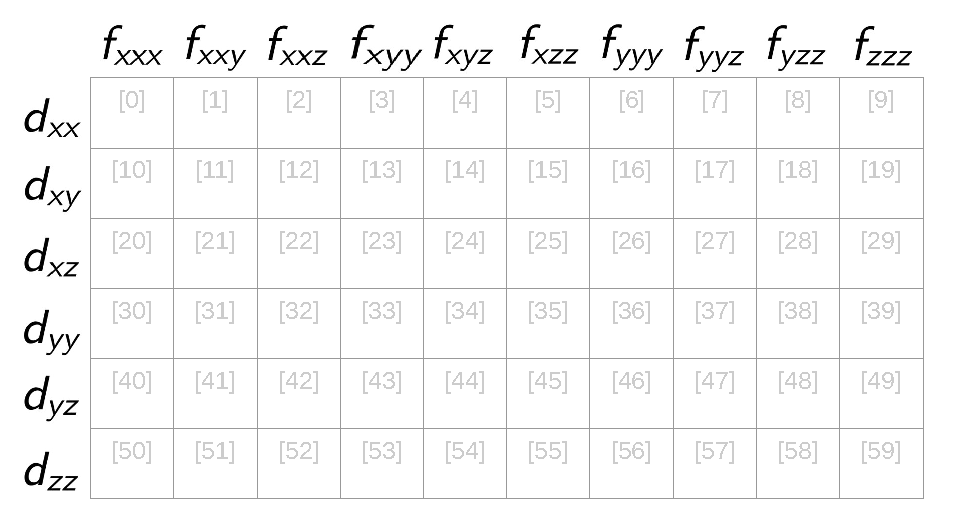
\includegraphics[width=0.45\textwidth]{d-f-matrix.pdf}
\caption{Molecular integrals calculated by \texttt{libgrpp} for the shell pair are stored in a one-dimensional array (here the special case of the $d$-$f$ shell pair is shown).}
\label{fig:dfmatrix}
\end{figure}


\subsection{Parametrization of pseudopotentials: \texttt{libgrpp\_potential\_t}}

For further use in molecular applications radial parts of GRPP components $U_L(r)$, $\Delta U_l(r)$, $U^{SO}_l(r)$ and $\Delta U_{n_clj}(r) = U_{n_clj}(r)-U_{lj}(r)$ (see Eq.~(\ref{eq:grpp-spin-orbital})) are expressed as linear combinations of radial Gaussian functions,
\begin{equation}
U(r) = \sum_k d_k r^{n_k-2} e^{-\zeta_k r^2},
\label{eq:param-potential}
\end{equation}
where $r$ stands for the distance from the point $\bm{C}$ at which the RPP is centered, $r = |\bm{r} - \bm{C}|$. The GRPPs for chemical elements from hydrogen to element 123 were derived from Dirac-Fock(-Breit) atomic calculations
in 1995--2022; the parameters $n_k$, $d_k$ and $\zeta_k$ were tabulated and can be found in~\cite{GRPP_website}.

The parametrization~(\ref{eq:param-potential}) is represented in \texttt{libgrpp} by the structure \texttt{libgrpp\_potential\_t}:
%
\begin{lstlisting}[language=C++]
typedef struct {
    int L;               // spatial angular momentum of the PP operator
    int J;               // total angular momentum of the PP operator
    int num_primitives;  // number of Gaussian primitives in the PP expansion
    int *powers;         // powers 'n' for each PP primitive
    double *coeffs;      // coefficients of the PP expansion
    double *alpha;       // exponents of the PP expansion
} libgrpp_potential_t;
\end{lstlisting}
%
Constructor and destructor for the \texttt{libgrpp\_potential\_t} object are defined as follows:
%
\begin{lstlisting}[language=C++]
libgrpp_potential_t *libgrpp_new_potential(
    int L,
    int J,
    int num_primitives,
    int *powers,
    double *coeffs,
    double *alpha
);

void libgrpp_delete_potential(libgrpp_potential_t *potential);
\end{lstlisting}


\subsection{Full GRPP object: \texttt{libgrpp\_grpp\_t}}
\label{sec:grpp-object}

The \texttt{libgrpp\_grpp\_t} structure represents the whole GRPP operator and includes all terms of the expansion~(\ref{eq:grpp-spin-orbital}):
%
\begin{lstlisting}[language=C++]
typedef struct {
    int n_arep;          // number of semilocal potentials in the scal-rel part
    int n_esop;          // number of potentials in the semilocal SO part
    int n_oc_shells;     // number of outercore shells / potentials
    libgrpp_potential_t *U_L;      // local potential U_L (r)
    libgrpp_potential_t **U_arep;  // list of scal -rel difference potentials
    libgrpp_potential_t **U_esop;  // list of effective SO potentials
    libgrpp_potential_t **U_oc;    // list of outercore potentials U_{n_c,lj}
    libgrpp_shell_t **oc_shells;   // list of outercore shells (for projectors)
} libgrpp_grpp_t;
\end{lstlisting}
%
Objects of type \texttt{libgrpp\_grpp\_t} are most conveniently constructed using the function:
%
\begin{lstlisting}[language=C++]
// constructor of the GRPP object
libgrpp_grpp_t * libgrpp_new_grpp ();
\end{lstlisting}
%
After the empty GRPP object is created, one can readily bind potentials and outercore shells to it:
%
\begin{lstlisting}[language=C++]
void libgrpp_grpp_set_local_potential(
    libgrpp_grpp_t *grpp, libgrpp_potential_t *pot
);

void libgrpp_grpp_add_averaged_potential(
    libgrpp_grpp_t *grpp, libgrpp_potential_t *pot
);

void libgrpp_grpp_add_spin_orbit_potential(
    libgrpp_grpp_t *grpp , libgrpp_potential_t *pot
);

// adds the pair (U_nlj, \phi_nlj) to GRPP
void libgrpp_grpp_add_outercore_potential(
    libgrpp_grpp_t *grpp , libgrpp_potential_t *pot , libgrpp_shell_t *oc_shell
);
\end{lstlisting}
%
To delete the \texttt{libgrpp\_grpp\_t} object and deallocate memory the destructor is provided:
%
\begin{lstlisting}[language=C++]
// destructor
void libgrpp_delete_grpp(libgrpp_grpp_t *grpp);
\end{lstlisting}
%
Please note that for the \texttt{libgrpp\_grpp\_t} object the semi-local spin-orbit potentials $U^{SO}_l(r)$ are multiplied by $\frac{2}{2l+1}$ \textit{inside} the \texttt{libgrpp} subroutines. This factor should not be accounted for during the construction of the \texttt{libgrpp\_grpp\_t} object!


\subsection{Initialization and finalization}

To be ready for calculations, \texttt{libgrpp} must be initialized. Initialization is needed to perform some pre-tabulations in a thread-safe manner. Optionally finalization can also be done at exit.

C interface:
%
\begin{lstlisting}[language=C++]
void libgrpp_init();
void libgrpp_finalize();
\end{lstlisting}

Fortran 90 interface:
%
\begin{lstlisting}[language=Fortran]
subroutine libgrpp_init()
subroutine libgrpp_finalize()
\end{lstlisting}


\subsection{Scalar-relativistic part: local potential integrals (type 1 integrals)}
\label{sec:type1-integrals}

Integrals over the local potential (type 1 integrals) are defined as:
%
\begin{equation}
\braket{\phi_A|U_L(r_C)|\phi_B}
\label{eq:def-type1-ints}
\end{equation}
%
Calculated matrix elements are stored in a one-dimensional array of type \texttt{double}, as it was shown on Fig.~\ref{fig:dfmatrix}. The array \texttt{matrix} must be pre-allocated.

C interface:
%
\begin{lstlisting}[language=C++]
void libgrpp_type1_integrals(
    libgrpp_shell_t *shell_A,
    libgrpp_shell_t *shell_B,
    double *rpp_origin,
    libgrpp_potential_t *potential,
    double *matrix
);
\end{lstlisting}

Fortran 90 interface:
%
\begin{lstlisting}[language=Fortran]
subroutine libgrpp_type1_integrals(                           &
    origin_A, L_A, num_primitives_A, coeffs_A, alpha_A,       &
    origin_B, L_B, num_primitives_B, coeffs_B, alpha_B,       &
    rpp_origin, rpp_nprim, rpp_powers, rpp_coeffs, rpp_alpha, &
    matrix                                                    & 
)

! shell centered on atom A
real(8)    :: origin_A(*)       ! point at which the basis function is centered
integer(4) :: L_A               ! angular momentum of the basis function
integer(4) :: num_primitives_A  ! number of Gaussian primitives
real(8)    :: coeffs_A(*)       ! contraction coefficients
real(8)    :: alpha_A(*)        ! exponents of Gaussian primitives

! shell centered on atom B
real(8)    :: origin_B(*)
integer(4) :: L_B
integer(4) :: num_primitives_B
real(8)    :: coeffs_B(*)
real(8)    :: alpha_B(*)

! pseudopotential expansion
real(8)    :: rpp_origin(*) ! point at which the PP is centered
integer(4) :: rpp_nprim     ! number of Gaussian primitives in the PP expansion
integer(4) :: rpp_powers(*) ! powers 'n' for each PP primitive
real(8)    :: rpp_coeffs(*) ! coefficients of the PP expansion
real(8)    :: rpp_alpha(*)  ! exponents of the PP expansion

! output: PP matrix elements
real(8)    :: matrix(*)
\end{lstlisting}
%

\subsection{Scalar-relativistic part: integrals with angular projectors (type 2 integrals)}

Integrals with angular projections (type 2 integrals) are defined as:
%
\begin{equation}
\braket{\phi_A|\Delta U_l(r_C) P_l|\phi_B}
\label{eq:def-type2-ints}
\end{equation}
%
The matrix array used to return matrix elements must be pre-allocated.

C interface:
%
\begin{lstlisting}[language=C++]
void libgrpp_type2_integrals(
    libgrpp_shell_t *shell_A,
    libgrpp_shell_t *shell_B,
    double *rpp_origin,
    libgrpp_potential_t *potential,
    double *matrix
);
\end{lstlisting}

Fortran 90 interface:
\begin{lstlisting}[language=Fortran]
subroutine libgrpp_type2_integrals(                                  &
    origin_A, L_A, num_primitives_A, coeffs_A, alpha_A,              &
    origin_B, L_B, num_primitives_B, coeffs_B, alpha_B,              &
    rpp_origin, rpp_L, rpp_nprim, rpp_powers, rpp_coeffs, rpp_alpha, &
    matrix                                                           &
)

! shell centered on atom A
real(8)    :: origin_A(*)       ! point at which the basis function is centered
integer(4) :: L_A               ! angular momentum of the basis function
integer(4) :: num_primitives_A  ! number of Gaussian primitives
real(8)    :: coeffs_A(*)       ! contraction coefficients
real(8)    :: alpha_A(*)        ! exponents of Gaussian primitives

! shell centered on atom B
real(8)    :: origin_B(*)
integer(4) :: L_B
integer(4) :: num_primitives_B
real(8)    :: coeffs_B(*)
real(8)    :: alpha_B(*)

! pseudopotential expansion
real(8)    :: rpp_origin(*) ! point at which the PP is centered
integer(4) :: rpp_L         ! angular momentum of the projector P_l
integer(4) :: rpp_nprim     ! number of Gaussian primitives in the PP expansion
integer(4) :: rpp_powers(*) ! powers 'n' for each PP primitive
real(8)    :: rpp_coeffs(*) ! coefficients of the PP expansion
real(8)    :: rpp_alpha(*)  ! exponents of the PP expansion

! output: PP matrix elements
real(8)    :: matrix (*)
\end{lstlisting}


\subsection{Effective spin-orbit interaction integrals}

Integrals over the effective spin-orbit interaction operator are defined as:
%
\begin{equation}
\braket{\phi_A|U^{SO}_l(r_C) P_l l_\eta|\phi_B}, \quad\quad \eta=x,y,z
\label{eq:def-so-ints}
\end{equation}
%
The \texttt{so\_x\_matrix}, \texttt{so\_y\_matrix} and \texttt{so\_z\_matrix} arrays used to return matrix elements must be preallocated. Note that the spin-orbit part in~(\ref{eq:grpp-spin-orbital}) also includes multiplication by the $ \bm{s} = \frac{1}{2}\bm{\sigma}$ operator. The factor $\frac{1}{2}$ is not accounted for by the \texttt{libgrpp} library. Multiplication by $2 \times 2$ Pauli matrices $\bm{\sigma}$ should be performed at the stage of the construction of the Hamiltonian matrix (see, for example,~\cite{Wuellen:10} for the detailed discussion).

C interface:
\begin{lstlisting}[language=C++]
void libgrpp_spin_orbit_integrals(
    libgrpp_shell_t *shell_A,
    libgrpp_shell_t *shell_B,
    double *rpp_origin,
    libgrpp_potential_t *potential,
    double *so_x_matrix,
    double *so_y_matrix,
    double *so_z_matrix
);
\end{lstlisting}

Fortran 90 interface:
\begin{lstlisting}[language=Fortran]
subroutine libgrpp_spin_orbit_integrals(                             &
    origin_A, L_A, num_primitives_A, coeffs_A, alpha_A,              &
    origin_B, L_B, num_primitives_B, coeffs_B, alpha_B,              &
    rpp_origin, rpp_L, rpp_nprim, rpp_powers, rpp_coeffs, rpp_alpha, &
    so_x_matrix, so_y_matrix, so_z_matrix                            &
)

! shell centered on atom A
real(8)    :: origin_A(*)       ! point at which the basis function is centered
integer(4) :: L_A               ! angular momentum of the basis function
integer(4) :: num_primitives_A  ! number of Gaussian primitives
real(8)    :: coeffs_A(*)       ! contraction coefficients
real(8)    :: alpha_A(*)        ! exponents of Gaussian primitives

! shell centered on atom B
real(8)    :: origin_B(*)
integer(4) :: L_B
integer(4) :: num_primitives_B
real(8)    :: coeffs_B(*)
real(8)    :: alpha_B(*)

! pseudopotential expansion
real(8)    :: rpp_origin(*) ! point at which the PP is centered
integer(4) :: rpp_L         ! angular momentum of the projector P_l
integer(4) :: rpp_nprim     ! number of Gaussian primitives in the PP expansion
integer(4) :: rpp_powers(*) ! powers 'n' for each PP primitive
real(8)    :: rpp_coef(*)   ! coefficients of the PP expansion
real(8)    :: rpp_alpha(*)  ! exponents of the PP expansion

! output: PP matrix elements for the X, Y, Z components
real(8)    :: so_x_matrix(*)
real(8)    :: so_y_matrix(*)
real(8)    :: so_z_matrix(*)
\end{lstlisting}



\subsection{GRPP-specific non-local part: integrals with projectors onto outercore shells}

Non-local GRPP-specific contributions to scalar-relativistic integrals
%
\begin{equation}
\braket{\phi_A|\sum_{l=0}^L \sum_{n_c} U^{AREP}_{n_c l}(r_C) P_l|\phi_B}
\label{eq:def-ocpot-arep-ints}
\end{equation}
%
and effective spin-orbit interaction
%
\begin{equation}
\braket{\phi_A|\sum_{l=1}^L \sum_{n_c} U^{SO}_{n_c l}(r_C) P_l l_\eta|\phi_B}, \quad\quad \eta=x,y,z
\label{eq:def-ocpot-so-ints}
\end{equation}
%
are calculated in \texttt{libgrpp} simultaneously. To construct these integrals via the formulas~(\ref{eq:nonlocal-arep})--(\ref{eq:nonlocal-operator-v}) one has to pass the list of outercore (difference) potentials $\Delta U_{n_c lj}(r) = U_{n_c lj}(r) - U_{lj}(r)$ and outercore pseudospinors $\tilde{\phi}_{n_c lj}$ to the integrator. Note the presence of the factor $\frac{2}{2l+1}$ in the formula~(\ref{eq:nonlocal-so}); thus the outercore potentials $\Delta U_{n_c lj}(r)$ are used directly and must not be pre-multiplied by this factor outside of \texttt{libgrpp}. Outercore shells $\tilde{\phi}_{n_c lj}$ are centered at the same point $\bm{C}$ as the GRPP operator.

C interface:
\begin{lstlisting}[language=C++]
void libgrpp_outercore_potential_integrals(
    libgrpp_shell_t *shell_A,
    libgrpp_shell_t *shell_B,
    double *rpp_origin,
    int num_oc_shells,
    libgrpp_potential_t **oc_potentials,
    libgrpp_shell_t **oc_shells,
    double *arep_matrix,
    double *so_x_matrix,
    double *so_y_matrix,
    double *so_z_matrix
);
\end{lstlisting}

Fortran 90 interface:
\begin{lstlisting}[language=Fortran]
subroutine libgrpp_outercore_potential_integrals(        &
    origin_A, L_A, num_primitives_A, coeffs_A, alpha_A,  &
    origin_B, L_B, num_primitives_B, coeffs_B, alpha_B,  &
    rpp_origin, num_oc_shells, oc_shells_L, oc_shells_J, &
    rpp_nprim, rpp_powers, rpp_coeffs, rpp_alpha,        &
    oc_shells_nprim, oc_shells_coeffs, oc_shells_alpha,  &
    arep_matrix, so_x_matrix, so_y_matrix, so_z_matrix   &
)

! shell centered on atom A
real(8)    :: origin_A(*)       ! point at which the basis function is centered
integer(4) :: L_A               ! angular momentum of the basis function
integer(4) :: num_primitives_A  ! number of Gaussian primitives
real(8)    :: coeffs_A(*)       ! contraction coefficients
real(8)    :: alpha_A(*)        ! exponents of Gaussian primitives

! shell centered on atom B
real(8)    :: origin_B(*)
integer(4) :: L_B
integer(4) :: num_primitives_B
real(8)    :: coeffs_B(*)
real(8)    :: alpha_B(*)

! pseudopotential expansion
real(8)    :: rpp_origin(*)    ! point at which the GRPP is centered
integer(4) :: num_oc_shells    ! total number of outercore potentials U_{n_c,lj}
integer(4) :: oc_shells_L(:)   ! angular momenta L of each outercore potential
integer(4) :: oc_shells_J(:)   ! total momenta J of each outercore potential
integer(4) :: rpp_nprim(:)     ! number of primitives for each OC potential
integer(4) :: rpp_powers(:, :) ! array of powers 'n' for each OC potential
real(8)    :: rpp_coeffs(:, :) ! expansion coeff-s for each OC potential
real(8)    :: rpp_alpha(:, :)  ! exponential parameters for each OC potential

! outercore shells used to construct projectors
integer(4) :: oc_shells_nprim(:)     ! number of primitives for each OC shell
real(8)    :: oc_shells_coeffs(:, :) ! contraction coeff-s for each OC shell
real(8)    :: oc_shells_alpha(:, :)  ! exponents of primitives for each OC shell

! output: PP matrix elements
! scalar-relativistic and spin-orbit parts are constructed simultaneously
real(8)    :: arep_matrix(*)
real(8)    :: so_x_matrix(*)
real(8)    :: so_y_matrix(*)
real(8)    :: so_z_matrix(*)
\end{lstlisting}


\subsection{Integrals over the full GRPP operator}

As it was described in Sect.~\ref{sec:grpp-object}, within the C interface the GRPP operator can be represented as an object of type \texttt{libgrpp\_grpp\_t}. Such an object can be passed to the routine \texttt{libgrpp\_full\_grpp\_integrals()}.

C interface:
\begin{lstlisting}[language=C++]
void libgrpp_full_grpp_integrals(
    libgrpp_shell_t *shell_A,
    libgrpp_shell_t *shell_B,
    libgrpp_grpp_t *grpp_operator,
    double *grpp_origin,
    double *arep_matrix,
    double *so_x_matrix,
    double *so_y_matrix,
    double *so_z_matrix
);
\end{lstlisting}
%
In this case both the scalar-relativistic parts and effective spin-orbit operator are integrated simultaneously.


\subsection{Analytic gradients of GRPP integrals}

\texttt{libgrpp} provides the possibility of calculation of analytic first derivatives of GRPP integrals with respect to nuclear coordinates. The algorithm was described in details in~\cite{Oleynichenko:LIBGRPP:23}. It is based on the property of the translational invariance of GRPP integrals and is exactly the same as in the case of ordinary semi-local pseudopotentials~\cite{Breidung:88,Russo:95,Cui:96,Bode:99,Song:15}. Analytic derivatives of GRPP integrals can be calculated most easily via the C interface, however, the Fortran interface is also available (see Sec.~\ref{sec:type1-grad}~--~\ref{sec:spin-orbit-grad}). The C routine employs the \texttt{libgrpp\_grpp\_t} object:
\begin{lstlisting}[language=C++]
void libgrpp_full_grpp_integrals_gradient(
    libgrpp_shell_t *shell_A,
    libgrpp_shell_t *shell_B,
    libgrpp_grpp_t *grpp_operator,
    double *grpp_origin,
    double *point_3d,
    double **grad_arep,
    double **grad_so_x,
    double **grad_so_y,
    double **grad_so_z
);
\end{lstlisting}
Differentiation is performed with respect to the 3D point \texttt{point\_3d}. Gradients with respect to each of the three spatial coordinates $x$, $y$, $z$ are stored in the \texttt{grad\_*} arrays. For example, \texttt{grad\_arep} contains pointers to three arrays:
\begin{equation}
\frac{\partial}{\partial P_x} \braket{\phi_A|\hat{U}^{GRPP}_C|\phi_B},\quad\quad
\frac{\partial}{\partial P_y} \braket{\phi_A|\hat{U}^{GRPP}_C|\phi_B},\quad\quad
\frac{\partial}{\partial P_z} \braket{\phi_A|\hat{U}^{GRPP}_C|\phi_B},
\end{equation}
where $\bm{P} = \{ P_x, P_y, P_z \}$ stands for the point with respect to the coordinates of which differentiation is performed (the same for the SO part). Overall 12 arrays of partial derivatives of matrix elements are returned
by the routine. Note that the \texttt{grad\_*} arrays must be pre-allocated before the invocation of the subroutine.

One can also use separate routines to evaluate gradients of different parts (local, semi-local, non-local) of GRPPs, see below.

\subsubsection{Analytic gradients: type 1 integrals}
\label{sec:type1-grad}

C interface:

\begin{lstlisting}[language=C++]
void libgrpp_type1_integrals_gradient(
    libgrpp_shell_t *shell_A,
    libgrpp_shell_t *shell_B,
    double *grpp_origin,
    libgrpp_potential_t *potential,
    double *point_3d,
    double **grad_arep
);
\end{lstlisting}

\noindent
Fortran 90 interface:

\begin{lstlisting}[language=Fortran]
subroutine libgrpp_type1_integrals_gradient(                           &
    origin_A, L_A, num_primitives_A, coeffs_A, alpha_A,                &
    origin_B, L_B, num_primitives_B, coeffs_B, alpha_B,                &
    rpp_origin, rpp_num_primitives, rpp_powers, rpp_coeffs, rpp_alpha, &
    point_3d, grad_arep_x, grad_arep_y, grad_arep_z                    &
)

! differentiation wrt the 3d point (x,y,z)
real(8), dimension(*), intent(in)  :: point_3d

! output: matrices d<Int>/dx, d<Int>/dy, d<Int>/dZ
real(8), dimension(*), intent(out) :: grad_arep_x
real(8), dimension(*), intent(out) :: grad_arep_y
real(8), dimension(*), intent(out) :: grad_arep_z
\end{lstlisting}
Other parameters of the Fortran subroutine are the same as for the \texttt{libgrpp\_type1\_integrals} subroutine for type 1 integrals, see Sec.~\ref{sec:type1-integrals}.

\subsubsection{Analytic gradients: type 2 integrals}
\label{sec:type2-grad}

C interface:

\begin{lstlisting}[language=C++]
void libgrpp_type2_integrals_gradient(
    libgrpp_shell_t *shell_A,
    libgrpp_shell_t *shell_B,
    double *grpp_origin,
    libgrpp_potential_t *potential,
    double *point_3d,
    double **grad_arep
);
\end{lstlisting}

\noindent
Fortran 90 interface:

\begin{lstlisting}[language=Fortran]
subroutine libgrpp_type2_integrals_gradient(            &
    origin_A, L_A, num_primitives_A, coeffs_A, alpha_A, &
    origin_B, L_B, num_primitives_B, coeffs_B, alpha_B, &
    rpp_origin, rpp_ang_momentum, rpp_num_primitives,   &
    rpp_powers, rpp_coeffs, rpp_alpha,                  &
    point_3d, grad_arep_x, grad_arep_y, grad_arep_z     &
)

! differentiation wrt the 3d point (x,y,z)
real(8), dimension(*), intent(in)  :: point_3d

! output: matrices d<Int>/dx, d<Int>/dy, d<Int>/dZ
real(8), dimension(*), intent(out) :: grad_arep_x
real(8), dimension(*), intent(out) :: grad_arep_y
real(8), dimension(*), intent(out) :: grad_arep_z
\end{lstlisting}

\subsubsection{Analytic gradients: spin-orbit integrals}
\label{sec:spin-orbit-grad}

C interface:

\begin{lstlisting}[language=C++]
void libgrpp_spin_orbit_integrals_gradient(
    libgrpp_shell_t *shell_A,
    libgrpp_shell_t *shell_B,
    double *grpp_origin,
    libgrpp_potential_t *potential,
    double *point_3d,
    double **grad_so_x,
    double **grad_so_y,
    double **grad_so_z
);
\end{lstlisting}

\noindent
Fortran 90 interface:

\begin{lstlisting}[language=Fortran]
subroutine libgrpp_spin_orbit_integrals_gradient(       &
    origin_A, L_A, num_primitives_A, coeffs_A, alpha_A, &
    origin_B, L_B, num_primitives_B, coeffs_B, alpha_B, &
    rpp_origin, rpp_ang_momentum, rpp_num_primitives,   &
    rpp_powers, rpp_coeffs, rpp_alpha,                  &
    point_3d, grad_sox_x, grad_sox_y, grad_sox_z,       &
    grad_soy_x, grad_soy_y, grad_soy_z,                 &
    grad_soz_x, grad_soz_y, grad_soz_z                  &
)

! differentiation wrt the 3d point (x,y,z)
real(8), dimension(*), intent(in)  :: point_3d

! output
! matrices d<SO_x>/dx, d<SO_x>/dy, d<SO_x>/dZ
real(8), dimension(*), intent(out) :: grad_sox_x
real(8), dimension(*), intent(out) :: grad_sox_y
real(8), dimension(*), intent(out) :: grad_sox_z

! matrices d<SO_y>/dx, d<SO_y>/dy, d<SO_y>/dZ
real(8), dimension(*), intent(out) :: grad_soy_x
real(8), dimension(*), intent(out) :: grad_soy_y
real(8), dimension(*), intent(out) :: grad_soy_z

! matrices d<SO_z>/dx, d<SO_z>/dy, d<SO_z>/dZ
real(8), dimension(*), intent(out) :: grad_soz_x
real(8), dimension(*), intent(out) :: grad_soz_y
real(8), dimension(*), intent(out) :: grad_soz_z
\end{lstlisting}

\section{Other one-electron integrals}

\subsection{Overlap integrals}

\begin{equation}
\braket{\phi_A|\phi_B}
\end{equation}

C interface:
\begin{lstlisting}[language=C++]
void libgrpp_overlap_integrals(
    libgrpp_shell_t *shell_A,
    libgrpp_shell_t *shell_B,
    double *overlap_matrix
);
\end{lstlisting}

Fortran 90 interface:
\begin{lstlisting}[language=Fortran]
subroutine libgrpp_overlap_integrals(                   &
    origin_A, L_A, num_primitives_A, coeffs_A, alpha_A, &
    origin_B, L_B, num_primitives_B, coeffs_B, alpha_B, &
    overlap_matrix                                      &
)

! shell centered on atom A
real(8)    :: origin_A(*)       ! point at which the basis function is centered
integer(4) :: L_A               ! angular momentum of the basis function
integer(4) :: num_primitives_A  ! number of Gaussian primitives
real(8)    :: coeffs_A(*)       ! contraction coefficients
real(8)    :: alpha_A(*)        ! exponents of Gaussian primitives

! shell centered on atom B
real(8)    :: origin_B(*)
integer(4) :: L_B
integer(4) :: num_primitives_B
real(8)    :: coeffs_B(*)
real(8)    :: alpha_B(*)

! output
real(8)    :: overlap_matrix(*)
\end{lstlisting}


\subsection{Kinetic-energy integrals}

\begin{equation}
\braket{\phi_A|-\frac{\Delta}{2}|\phi_B}
\end{equation}

C interface:
\begin{lstlisting}[language=C++]
void libgrpp_kinetic_energy_integrals(
    libgrpp_shell_t *shell_A,
    libgrpp_shell_t *shell_B,
    double *kinetic_matrix
);
\end{lstlisting}

Fortran 90 interface:
\begin{lstlisting}[language=Fortran]
subroutine libgrpp_kinetic_energy_integrals(            &
    origin_A, L_A, num_primitives_A, coeffs_A, alpha_A, &
    origin_B, L_B, num_primitives_B, coeffs_B, alpha_B, &
    kinetic_matrix                                      &
)

! shell centered on atom A
real(8)    :: origin_A(*)       ! point at which the basis function is centered
integer(4) :: L_A               ! angular momentum of the basis function
integer(4) :: num_primitives_A  ! number of Gaussian primitives
real(8)    :: coeffs_A(*)       ! contraction coefficients
real(8)    :: alpha_A(*)        ! exponents of Gaussian primitives

! shell centered on atom B
real(8)    :: origin_B(*)
integer(4) :: L_B
integer(4) :: num_primitives_B
real(8)    :: coeffs_B(*)
real(8)    :: alpha_B(*)

! output
real(8)    :: kinetic_matrix(*)
\end{lstlisting}


\subsection{Momentum integrals}

\begin{equation}
\braket{\phi_A|-i\nabla|\phi_B} = 
-i \left(
\braket{\phi_A|\frac{\partial}{\partial x}|\phi_B},
\braket{\phi_A|\frac{\partial}{\partial y}|\phi_B},
\braket{\phi_A|\frac{\partial}{\partial z}|\phi_B}
\right)
\end{equation}

Subroutines return imaginary parts on momentum integrals, the ``minus'' sign is accounted for.

C interface:
\begin{lstlisting}[language=C++]
void libgrpp_momentum_integrals(
    libgrpp_shell_t *shell_A,
    libgrpp_shell_t *shell_B,
    double *px_matrix,
    double *py_matrix,
    double *pz_matrix
);
\end{lstlisting}

Fortran 90 interface:
\begin{lstlisting}[language=Fortran]
subroutine libgrpp_momentum_integrals(                  &
    origin_A, L_A, num_primitives_A, coeffs_A, alpha_A, &
    origin_B, L_B, num_primitives_B, coeffs_B, alpha_B, &
    px_matrix, py_matrix, pz_matrix                     &
)

! shell centered on atom A
real(8)    :: origin_A(*)       ! point at which the basis function is centered
integer(4) :: L_A               ! angular momentum of the basis function
integer(4) :: num_primitives_A  ! number of Gaussian primitives
real(8)    :: coeffs_A(*)       ! contraction coefficients
real(8)    :: alpha_A(*)        ! exponents of Gaussian primitives

! shell centered on atom B
real(8)    :: origin_B(*)
integer(4) :: L_B
integer(4) :: num_primitives_B
real(8)    :: coeffs_B(*)
real(8)    :: alpha_B(*)

! output
real(8)    :: px_matrix(*)
real(8)    :: py_matrix(*)
real(8)    :: pz_matrix(*)
\end{lstlisting}

\subsection{Nuclear attraction integrals}

\texttt{libgrpp} includes routines for evaluation of multi-center one-electron integrals over electrostatic potentials generated by different nuclear charge distribution models. Particular nuclear model is specified by one of the
predefined constants listed below:

\begin{itemize}
\item \texttt{LIBGRPP\_NUCLEAR\_MODEL\_POINT\_CHARGE = 0}

Point nucleus:
\begin{equation}
V = -\frac{Z}{r}
\end{equation}

\item \texttt{LIBGRPP\_NUCLEAR\_MODEL\_CHARGED\_BALL = 1}

Uniformly charged ball model. The charge density $\rho(r)$ is given by~\cite{Visscher:97}:
\begin{equation}
\rho^U(r) = \begin{cases}
\rho_0 = \frac{3Z}{4\pi R^3_0}, & r \le R_0, \\
0, & r > R_0.
\end{cases}
\end{equation}
The charged ball radius R0 is connected with the root mean square radius $R_{rms} = \braket{r^2}^{1/2}$ by the relation:
\begin{equation}
R_0 = \sqrt{\frac{5}{3}}\ R_{rms}
\end{equation}

\item \texttt{LIBGRPP\_NUCLEAR\_MODEL\_GAUSSIAN = 2}

Gaussian distribution model~\cite{Visscher:97}:
\begin{equation}
\rho^G(r) = Z \left( \frac{\xi}{\pi} \right)^{3/2} e^{-\xi r^2}
\end{equation}
\begin{equation}
\xi = \frac{3}{2 R_{rms}^2}
\end{equation}

\item \texttt{LIBGRPP\_NUCLEAR\_MODEL\_FERMI = 3}

Fermi distribution model~\cite{Visscher:97,Parpia:92,Mosyagin:20}:
\begin{equation}
\rho^F(r) = \frac{\rho_0}{1 + \exp(\frac{r-c}{a})}
\end{equation}
The $c$ parameter is related to $R_{rms}$ by the approximate relation:
\begin{equation}
c^2 = \frac{5}{3}R^2_{rms} - \frac{7}{3}\pi^2 a^2.
\end{equation}

\item \texttt{LIBGRPP\_NUCLEAR\_MODEL\_FERMI\_BUBBLE = 4}

The extension of the Fermi model for the ``bubble''-type nuclei with the lowering of charge density at $r = 0$ (``a hole in the origin'')~\cite{Flambaum:19}:
\begin{equation}
\rho^F(r) = \left( 1 + k \frac{r^2}{c^2} \right) \frac{\rho_0}{1 + \exp(\frac{r-c}{a})}
\end{equation}
Analytic formulas underlying this model (including that for $R_{rms}$) either can be found in the source code or are available under request.
\end{itemize}

C interface:
\begin{lstlisting}[language=C++]
void libgrpp_nuclear_attraction_integrals(
    libgrpp_shell_t *shell_A,
    libgrpp_shell_t *shell_B,
    double *charge_origin,
    int charge,
    int nuclear_model,
    double *model_params,
    double *coulomb_matrix
);
\end{lstlisting}

The \texttt{nuclear\_model} argument should be equal to one of the constants listed above. The \texttt{model\_params[]} argument is used to pass parameters of the nuclear models. All model parameters must be given in bohrs.
\begin{itemize}
\item Point nucleus: is not used;
\item Uniformly charged ball:

\texttt{model\_params = [R\_rms]}
\item Gaussian model:

\texttt{model\_params = [R\_rms]}
\item Fermi model:

\texttt{model\_params = [c,a]}
\item Fermi model with a hole (``bubble''):

\texttt{model\_params = [c,a,k]}
\end{itemize}

Fortran 90 interface:
\begin{lstlisting}[language=Fortran]
subroutine libgrpp_nuclear_attraction_integrals(        &
    origin_A, L_A, num_primitives_A, coeffs_A, alpha_A, &
    origin_B, L_B, num_primitives_B, coeffs_B, alpha_B, &
    charge_origin, charge, nuclear_model, model_params, &
    matrix                                              &
)

! shell centered on atom A
real(8)    :: origin_A(*)       ! point at which the basis function is centered
integer(4) :: L_A               ! angular momentum of the basis function
integer(4) :: num_primitives_A  ! number of Gaussian primitives
real(8)    :: coeffs_A(*)       ! contraction coefficients
real(8)    :: alpha_A(*)        ! exponents of Gaussian primitives

! shell centered on atom B
real(8)    :: origin_B(*)
integer(4) :: L_B
integer(4) :: num_primitives_B
real(8)    :: coeffs_B(*)
real(8)    :: alpha_B(*)

! nuclear potential definition
real(8)    :: charge_origin(*)
integer(4) :: charge
integer(4) :: nuclear_model
real(8)    :: model_params(*)

! output
real(8)    :: matrix(*)
\end{lstlisting}

In addition, specialized subroutines can be used:
\begin{lstlisting}[language=C++]
void libgrpp_nuclear_attraction_integrals_point_charge(
    libgrpp_shell_t *shell_A,
    libgrpp_shell_t *shell_B,
    double *charge_origin,
    int charge,
    double *coulomb_matrix
);
\end{lstlisting}

\begin{lstlisting}[language=C++]
void libgrpp_nuclear_attraction_integrals_charged_ball(
    libgrpp_shell_t *shell_A,
    libgrpp_shell_t *shell_B,
    double *charge_origin,
    int charge,
    double r_rms,
    double *coulomb_matrix
);
\end{lstlisting}

\begin{lstlisting}[language=C++]
void libgrpp_nuclear_attraction_integrals_gaussian_model(
    libgrpp_shell_t *shell_A,
    libgrpp_shell_t *shell_B,
    double *charge_origin,
    int charge,
    double r_rms,
    double *coulomb_matrix
);
\end{lstlisting}

\begin{lstlisting}[language=C++]
void libgrpp_nuclear_attraction_integrals_fermi_model(
    libgrpp_shell_t *shell_A,
    libgrpp_shell_t *shell_B,
    double *charge_origin,
    int charge,
    double fermi_param_c,
    double fermi_param_a,
    double *coulomb_matrix
);
\end{lstlisting}

\begin{lstlisting}[language=C++]
void libgrpp_nuclear_attraction_integrals_fermi_bubble_model(
    libgrpp_shell_t *shell_A,
    libgrpp_shell_t *shell_B,
    double *charge_origin,
    int charge,
    double param_c,
    double param_a,
    double param_k,
    double *coulomb_matrix
);
\end{lstlisting}

Fortran 90 interface is the same as for the \texttt{libgrpp\_nuclear\_attraction\_integrals()} subroutine.


\section{Programming examples}

\texttt{libgrpp} provides two simple demonstration programs, \texttt{test\_libgrpp\_c} and \texttt{test\_libgrpp\_f90}. These programs illustrate how to call the \texttt{libgrpp} routines. Here we present the most important code samples in both C and Fortran languages. Note that \texttt{libgrpp} should not be initialized before the use; this initialization
is implicit and is performed the first time when the library is accessed from the client code.

\emph{\color{red}Do not forget to invoke the \texttt{libgrpp\_init()} subroutine for initialization before any other calls to the \texttt{libgrpp} interface!}

\subsection{Example: C}

The following listing shows how to construct integrals over the full GRPP operator for the given list of several basis shells.

\begin{lstlisting}[language=C++]
// ... some other useful headers ...
#include "../libgrpp/libgrpp.h"

#define MAX_BUF 10000

/**
 * evaluates matrix elements of the GRPP operator
 */
void evaluate_grpp_integrals(
    int num_shells, libgrpp_shell_t **shell_list,
    molecule_t *molecule, libgrpp_grpp_t **grpp_list,
    double *arep_matrix,
    double *so_x_matrix,
    double *so_y_matrix,
    double *so_z_matrix
)
{
    // buffers used to store matrix elements for a shell pair
    double buf_arep[MAX_BUF];
    double buf_spin_orbit[3][MAX_BUF];
    
    int dim = calculate_basis_dim(shell_list, num_shells);

    // square matrices used to store matrix elements for the whole molecule
    memset(arep_matrix, 0, sizeof(double) * dim * dim);
    memset(so_x_matrix, 0, sizeof(double) * dim * dim);
    memset(so_y_matrix, 0, sizeof(double) * dim * dim);
    memset(so_z_matrix, 0, sizeof(double) * dim * dim);

    // loop over bra shells
    int ioffset = 0;
    for (int ishell = 0; ishell < num_shells; ishell++) {

        libgrpp_shell_t *bra = shell_list[ishell];
        int bra_dim = libgrpp_get_shell_size(bra);

        // loop over ket shells
        int joffset = 0;
        for (int jshell = 0; jshell < num_shells; jshell++) {
        
            libgrpp_shell_t *ket = shell_list[jshell];
            int ket_dim = libgrpp_get_shell_size(ket);

            // loop over atoms; GRPPs are provided only for the part of atoms
            for (int iatom = 0; iatom < molecule->n_atoms; iatom++) {
                int z = molecule->charges[iatom];
                libgrpp_grpp_t *grpp = grpp_list[z];
                if (grpp == NULL) {
                    continue;
                }
                
                double ecp_origin[3];
                ecp_origin[0] = molecule->coord_x[iatom];
                ecp_origin[1] = molecule->coord_y[iatom];
                ecp_origin[2] = molecule->coord_z[iatom];

                evaluate_grpp_integrals_shell_pair(
                    bra, ket, grpp, ecp_origin, buf_arep,
                    buf_spin_orbit[0], buf_spin_orbit[1], buf_spin_orbit[2]
                );
                
                // the rectangular block of matrix elements is added to the
                // resulting square matrix
                add_block_to_matrix (dim, dim, arep_matrix, bra_dim, ket_dim,
                    buf_arep, ioffset, joffset, 1.0);
                add_block_to_matrix(dim, dim, so_x_matrix, bra_dim, ket_dim,
                    buf_spin_orbit[0], ioffset, joffset, 1.0);
                add_block_to_matrix(dim, dim, so_y_matrix, bra_dim, ket_dim,
                    buf_spin_orbit[1], ioffset, joffset, 1.0);
                add_block_to_matrix(dim, dim, so_z_matrix, bra_dim, ket_dim,
                    buf_spin_orbit[2], ioffset, joffset, 1.0);
            }
            
            joffset += ket_dim ;
        }
        
        ioffset += bra_dim ;
    }
}
\end{lstlisting}

The subroutine \texttt{evaluate\_grpp\_integrals\_shell\_pair()} evaluating GRPP matrix elements for the pair of shells is given by the following code:

\begin{lstlisting}[language=C++]
void evaluate_grpp_integrals_shell_pair(
    libgrpp_shell_t *shell_A,
    libgrpp_shell_t *shell_B,
    libgrpp_grpp_t *grpp_operator,
    double *grpp_origin,
    double *arep_matrix,
    double *so_x_matrix,
    double *so_y_matrix,
    double *so_z_matrix
)
{
    size_t size = shell_A->cart_size * shell_B->cart_size;
    double *buf_arep = (double *) calloc(size, sizeof(double));
    double *buf_so_x = (double *) calloc(size, sizeof(double));
    double *buf_so_y = (double *) calloc(size, sizeof(double));
    double *buf_so_z = (double *) calloc(size, sizeof(double));

    memset(arep_matrix, 0, sizeof(double) * size);
    memset(so_x_matrix, 0, sizeof(double) * size);
    memset(so_y_matrix, 0, sizeof(double) * size);
    memset(so_z_matrix, 0, sizeof(double) * size);

    /*
     * radially-local ("type-1") integrals
     */
    libgrpp_type1_integrals(
        shell_A, shell_B, grpp_origin, grpp_operator->U_L, buf_arep
    );
    update_vector(size, arep_matrix, 1.0, buf_arep);
    
    /*
     * semilocal AREP ("type-2") integrals
     */
    for (int L = 0; L < grpp_operator->n_arep; L++) {
        libgrpp_type2_integrals(
            shell_A, shell_B, grpp_origin, grpp_operator->U_arep[L], buf_arep
        );
        update_vector(size, arep_matrix, 1.0, buf_arep);
    }

    /*
     * semilocal SO (" type -3") integrals
     */
    for (int L = 1; L < grpp_operator->n_esop; L++) {
        libgrpp_spin_orbit_integrals(
            shell_A, shell_B, grpp_origin, grpp_operator->U_esop[L],
            buf_so_x, buf_so_y, buf_so_z
        );
        update_vector(size, so_x_matrix, 2.0 / (2 * L + 1), buf_so_x);
        update_vector(size, so_y_matrix, 2.0 / (2 * L + 1), buf_so_y);
        update_vector(size, so_z_matrix, 2.0 / (2 * L + 1), buf_so_z);
    }

    /*
     * integrals over outercore non-local potentials,
     * the part specific for GRPP.
     *
     * note that proper prefactors for the SO part are calculated inside
     * the libgrpp_outercore_potential_integrals() procedure.
     */
    libgrpp_outercore_potential_integrals(
        shell_A, shell_B, grpp_origin, grpp_operator->n_oc_shells,
        grpp_operator->U_oc, grpp_operator->oc_shells,
        buf_arep, buf_so_x, buf_so_y, buf_so_z
    );
    update_vector(size, arep_matrix, 1.0, buf_arep);
    update_vector(size, so_x_matrix, 1.0, buf_so_x);
    update_vector(size, so_y_matrix, 1.0, buf_so_y);
    update_vector(size, so_z_matrix, 1.0, buf_so_z);

    /*
     * cleanup
     */
    free(buf_arep);
    free(buf_so_x);
    free(buf_so_y);
    free(buf_so_z);
}
\end{lstlisting}


\subsection{Example: Fortran 90}

The code in Fortran 90 is more cumbersome, since the object-oriented features of modern Fortran were abandoned in \texttt{libgrpp} in order to preserve the interoperability with codes written in Fortran 77 (widely used in quantum chemistry software). The Fortran 90 interface of \texttt{libgrpp} is purely procedural. The following code snippets are taken from the source code of the \texttt{test\_libgrpp\_f90} sample program (see file \texttt{evalints.f90}). Consider, for example, the loop over shell pairs with the invocation of the subroutine \texttt{libgrpp\_spin\_orbit\_integrals()}:

\begin{lstlisting}[language=Fortran]
! initialization of the resulting matrices

arep_matrix = 0.0d0
so_matrices = 0.0d0

ioffs = 0
ishell = 0

! loop over shell pairs
do iatom1 = 1, natoms
  z1 = charges(iatom1) ! atomic charge is used to get the basis set
  do iblock1 = 1, num_blocks(z1)
    do ifun1 = 1, block_num_contr(z1, iblock1)
      call generate_cartesians(iblock1 - 1, cart_list_1, ncart1)
      ishell = ishell + 1
      
      joffs = 0
      jshell = 0
      do iatom2 = 1, natoms
        z2 = charges(iatom2)
        do iblock2 = 1, num_blocks(z2)
          do ifun2 = 1, block_num_contr(z2, iblock2)
            call generate_cartesians(iblock2 - 1, cart_list_2, ncart2)
            jshell = jshell + 1

            L_A = iblock1 - 1
            L_B = iblock2 - 1
            nprim_A = block_num_prim(z1, iblock1)
            nprim_B = block_num_prim(z2, iblock2)

            ! sum over atoms with pseudopotentials
            do ic = 1, natoms
              zc = charges(ic)
              if (n_arep(zc) == 0) then ! no RPP for this atom => skip it
                cycle
              end if

              ! radially-local part (type-1 integrals)
              ! ... the code ...

              ! semilocal averaged part (type-2 integrals )
              ! ... the code ...

              ! semilocal spin-orbit part
              do iarep = 2, n_arep(zc)
                L = iarep - 1
                call libgrpp_spin_orbit_integrals( &
                  coord(iatom1, :), L_A, nprim_A,  & ! basis shell 1
                  coeffs(z1, iblock1, ifun1, :), exponents(z1, iblock1, :), &
                  coord(iatom2, :), L_B, nprim_B,  & ! basis shell 2
                  coeffs(z2, iblock2, ifun2, :), exponents(z2, iblock2, :), &
                  coord(ic, :), L, ecp_num_prim(zc, iarep),     & ! potential
                  ecp_powers(zc, iarep, :), esop(zc, iarep, :), &
                  ecp_alpha(zc, iarep, :), buf_x, buf_y, buf_z  &
                )
                
                ! contributions to the SO interaction must be scaled
                ! since these factors are not accounted for in the input
                ! file format for GRPPs
                buf_x = buf_x * 2.0 / (2.0 * L + 1)
                buf_y = buf_y * 2.0 / (2.0 * L + 1)
                buf_z = buf_z * 2.0 / (2.0 * L + 1)
                call update_matrix_part(so_matrices(1,:,:), ioffs, joffs, &
                  buf_x, ncart1, ncart2)
                call update_matrix_part(so_matrices(2,:,:), ioffs, joffs, &
                  buf_y, ncart1, ncart2)
                call update_matrix_part(so_matrices(3,:,:), ioffs, joffs, &
                  buf_z, ncart1, ncart2)
              end do

              ! non-local part
              ! ... the code ...

              ! add the contribution of the given shell pair
              ! to the overall square RPP matrices
              call update_matrix_part(so_matrices(1,:,:), ioffs, joffs, &
                buf_x, ncart1, ncart2)
              call update_matrix_part(so_matrices(2,:,:), ioffs, joffs, &
                buf_y, ncart1, ncart2)
              call update_matrix_part(so_matrices(3,:,:), ioffs, joffs, &
                buf_z, ncart1, ncart2)

            end do

            joffs = joffs + ncart2

          end do
        end do
      end do

      ioffs = ioffs + ncart1
      
    end do
  end do
end do
\end{lstlisting}

This code is rather straightforward. It relies on parameters of RPPs and basis sets available in the global namespace (using the mechanism of Fortran 90 modules). Parameters of the basis sets are stored in several arrays defined in \texttt{basis.f90}:

\begin{lstlisting}[language=Fortran]
integer, parameter :: MAXL = 10
integer, parameter :: MAX_CNTRCT_LEN = 30

! basis set data
integer :: num_blocks(N_ELEMENTS)
integer :: block_num_prim(N_ELEMENTS, MAXL)
integer :: block_num_contr(N_ELEMENTS, MAXL)
real(8) :: exponents(N_ELEMENTS, MAXL, MAX_CNTRCT_LEN)
real(8) :: coeffs(N_ELEMENTS, MAXL, MAX_CNTRCT_LEN, MAX_CNTRCT_LEN)
\end{lstlisting}

Quite analogous structures are defined in \texttt{rpp.f90} to store parameters of (G)RPPs:

\begin{lstlisting}[language=Fortran]
integer, parameter :: ECP_MAXL = 10
integer, parameter :: ECP_MAX_CNTRCT_LEN = 50
integer, parameter :: ECP_MAX_OC_SHELLS = 20

! pseudopotential data
! number of partial-wave potentials for each element
integer :: n_arep(N_ELEMENTS)
integer :: n_esop(N_ELEMENTS)
integer :: n_oc_shells(N_ELEMENTS, ECP_MAXL)
integer :: ecp_num_prim(N_ELEMENTS, ECP_MAXL)

! parameters of RPP Gaussian expansions
real(8) :: ecp_alpha(N_ELEMENTS, ECP_MAXL, ECP_MAX_CNTRCT_LEN)
integer :: ecp_powers(N_ELEMENTS, ECP_MAXL, ECP_MAX_CNTRCT_LEN)
real(8) :: arep(N_ELEMENTS, ECP_MAXL, ECP_MAX_CNTRCT_LEN)
real(8) :: esop(N_ELEMENTS, ECP_MAXL, ECP_MAX_CNTRCT_LEN)
real(8) :: ocpot(N_ELEMENTS, ECP_MAXL, ECP_MAX_OC_SHELLS, ECP_MAX_CNTRCT_LEN)

! outercore basis set used to construct outercore projectors
! (GRPP-specific part)
integer :: ocbas_num_prim(N_ELEMENTS, ECP_MAXL)
integer :: ocbas_num_contr(N_ELEMENTS, ECP_MAXL)
real(8) :: ocbas_alpha(N_ELEMENTS, ECP_MAXL, ECP_MAX_CNTRCT_LEN)
real(8) :: ocbas_coeffs(N_ELEMENTS, ECP_MAXL, ECP_MAX_CNTRCT_LEN, &
  ECP_MAX_CNTRCT_LEN)
\end{lstlisting}

Of course, basis sets and pseudopotentials can be stored in any other way, since \texttt{libgrpp} subroutines expect only pointers to arrays containing these data.

\bibliography{manual}{}
\bibliographystyle{unsrt}

\end{document}

